\chapter{Software y Nube}\label{S:anexo_C}
Este anexo muestra el razonamiento detenido, la comparativa de pruebas de concepto realizadas en el anexo \ref{S:anexo_E} y configuración dentro del capitulo 2.

\section{Software}\label{S:decisiones_software}
El primer punto que debemos decidir\cite{c_inhouse_outsource} es la modalidad del tipo de servicios que queremos utilizar. Desde el punto de vista técnico, podemos optar entre la externalización o la autogestión, y llegado a un extremo la nube autócrata. Por otra parte, la licencia del software a utilizar así como la flexibilidad, customización y costes asociados difieren entre dos tipos de soluciones “la solución completa” dentro de un marco de trabajo (usualmente privado y de pago) o “soluciones concretas” que se integran con diferentes gestores y se basan comunidades auto documentadas (generalmente más económica y libre). 

\subsection{Proveedor, mantenimiento y gestión}
Externalizar significa utilizar un servicio público proveído por empresas ya sea en modalidad gratuita o de pago. Al ser un producto estándar conlleva ventajas y desventajas, no es customizable, pero facilita su uso y mantenimiento, siendo normalmente transparente al usuario. 

Auto gestionar sin embargo indica que aunque sea un producto estándar, la instalación, mantenimiento y solución de incidencias es propia. Requiere de un mayor conocimiento técnico y una dedicación semanal o mensual para tareas de mantenimiento o prevención, sin embargo además de una mayor customización y agilidad con las incidencias, usualmente es mucho más económico en términos generales.

La externalización se puede producir a diferentes niveles, la autogestión usualmente externaliza el hardware/servidor o la gestión de la máquina virtual pero mantiene y gestiona el software instalado. Un usuario puede decidir usar su propio hardware y su conexión a internet para generar una nube autócrata, pero cuya complejidad y mantenimiento a veces no la hace funcional, simplemente autócrata y debido al coste eléctrico asociado lo hace inviable económicamente hablando.

Finalmente se debe entender que a veces un software funciona como un servicio. Gestionar un servicio muchas veces no tiene que ver con el propio software sino con la escalabilidad, backups y transferencia del servicio a otro proveedor, por lo que la autogestión y \textbf{la externalización parcial deben ser fácilmente intercambiables}.

\subsection{Licencias y tipo de software}
Por otra parte, hay que decidir qué aplicativo usamos entre las múltiples posibilidades que ofrecen un resultado similar, pero cuyas características legales y técnicas cambian. 

Existen 5 propiedades intrínsecas a todo software:
\begin{itemize}
    \item Propiedad intelectual.
    \item Tipo de licencia de uso, distribución y/o modificación.
    \item Código abierto (publicado) o cerrado.
    \item Compatibilidad, requisitos o ecosistema integrado.
    \item Vida útil, refiere al mantenimiento, LTS, actualización del software. 
\end{itemize}

\begin{figure}[!htb]
\begin{center}
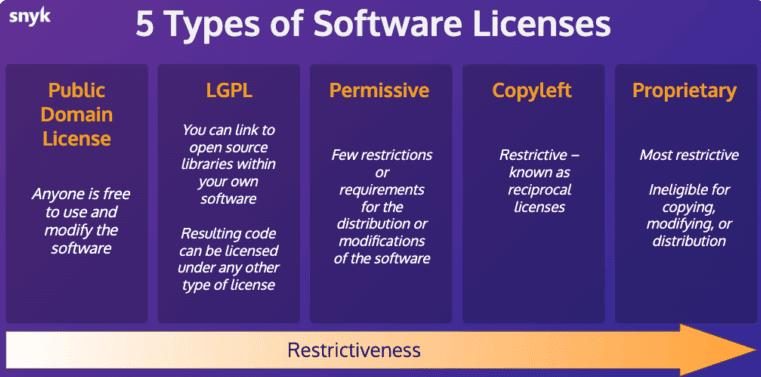
\includegraphics[width=0.9\textwidth]{./figuras/licencias.jpg}
\caption{Tipos de licencias mas comunes\cite{c_licencias}.}
\label{F:licencias}
\end{center}
\end{figure}

Obviando la casuística concreta de cada software, en una visión global se pueden distinguir dos bloques claros de tipos de software:

“Software privativo”, son aquellos cuyo propietario es una persona o empresa y el uso de dicho software requiere de licencia gratuita o de pago. Así como los requisitos del mismo depende de la compatibilidad realizada por el propietario.
Desde el punto de vista técnico, estos software pueden ser abiertos o cerrados indicando si el código que los construye es público/visible o no. Usualmente estos softwares son de pago, o licencias gratuitas bajo restricciones y suelen funcionar bajo entornos de trabajo privativos que unifican un conjunto de aplicaciones como solución interdisciplinar. Ejemplo entorno de trabajo Microsoft (azure, windows, office, github, atlassian solutions), entornos de trabajo Google(cloud, chromium OS, gmail, maps ...) .

“Software Libre”, es un término que hace referencia a la libertad para usarlo, estudiarlo, distribuirlo, adaptarlo o mejorar el programa. Estos software pueden ser tanto empresariales como realizados por comunidades o programadores independientes, en todos los casos los creadores del software siguen siendo sus propietarios, pero no existe restricciones a su uso o mejora, así como tienen licencias de coste cero. La principal ventajas de estos software son las comunidades y la facilidad de mejora del código al ser abierto. Por otra parte las empresas que colaboran o sustentan estas aplicaciones, ofrecen dichos software a precios competitivos, donde el coste está asociado a la infraestructura, gestión y mantenimiento del software no a la licencia en sí y normalmente permiten la existencia de un mercado de plugins, módulos o configuraciones extras proveídas tanto por empresas como programadores profesionales. Ejemplos: linux, libreoffice y aplicaciones web o frameworks (ubuntu, wordpress, prestashop, frameworks como laravel, angular, spring boot).

Actualmente existe una mayor popularidad de software libre en servidores, aunque por contra posición el mercado es mayoritariamente privativo en el segmento escritorio. Esto se debe especialmente al SO (Sistema Operativo) empleado en las diferentes plataformas que condicionan los ecosistemas utilizados.

\section{Elección de Servidor}\label{S:anexo_segurizacion}
El primer elemento necesario de nuestra cloud, es el servidor principal. Debido a que nuestro objetivo primario es la instalación de múltiples softwares y la gestión de los mismos, lo más intuitivo es el uso de un servidor o VPS (virtual private server) sin embargo otras opciones como la dockerización de servicios directamente por un proveedor también es una opción valida.

\subsection{Servidor Físico vs Servidor virtual vs Cloud Externo}
Existen dos opciones basadas en servidores físicos, la principal es la contratación a un proveedor de una máquina con características específicas; usualmente este tipo de servidores son de un coste alto y unos requisitos de hardware excesivos para nuestras necesidades. La secundaria el uso de VPS o servidores virtuales dinámicos no sólo permite reducir significativamente su coste, sino que también está asociados a un escalado dinámico (vertical) más flexible y en función de la demanda.

\begin{figure}[!htb]
\begin{center}
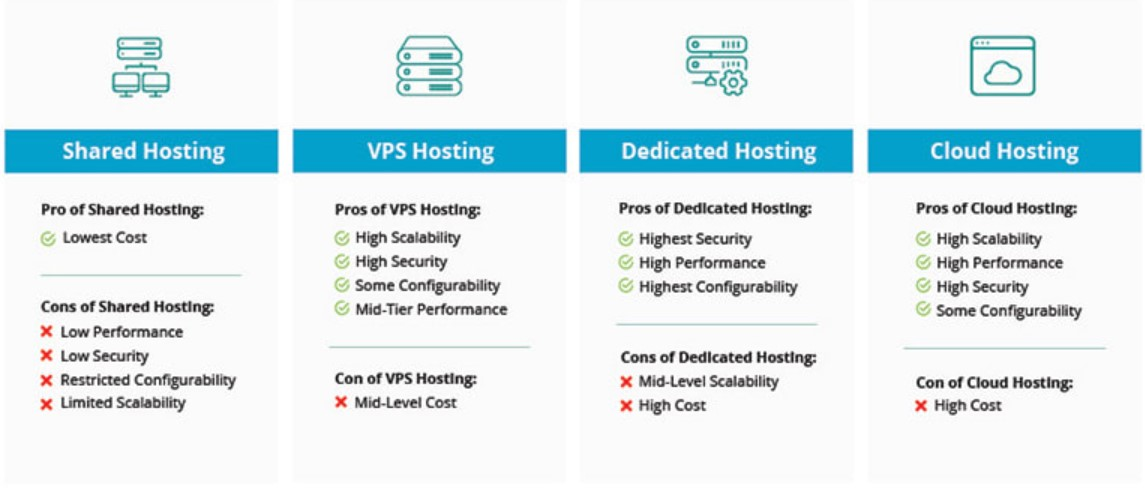
\includegraphics[width=1\textwidth]{./figuras/servidores_typos_servicios.jpg}
\caption{Tipos de servicios en servidores\cite{i_vps}.}
\label{F:servidores_typos_servicios}
\end{center}
\end{figure}

La alternativa es el uso de un servidor propio instalado, en la “oficina real”. Obviando el hecho de la compra del hardware o el reuso de un pc para dichos fines, requiere de una conexión a internet alta velocidad y simétrica (fibra) y un consumo eléctrico continuado. Dependiendo del ISP(Internet Service Provider), existirá un problema de IP dinámica, puerto dinámico o servicio de pago para la obtención de IP estática, incluso la no existencia de una ip pública por CG-Nat\cite{c_cg_nat}.

\begin{table}[!ht]
    \centering
    \label{T:tipos_servidores}
    \caption{Tabla comparativa opciones servidor.}    
    \begin{tabular}{|p{3cm}|p{3.5cm}|p{3.5cm}|p{3cm}|}
    \hline \hline
        \textbf{Tipo de solución} & \textbf{Ventajas} & \textbf{Desventajas} & \textbf{Coste} \\ \hline
        Virtual Private server (bajos recursos) & Externalizado, alta disponibilidad, escalabilidad y migración & Servicios de backup costoso. Recursos limitados & 3-15 € / mes \\ \hline
        Dedicated Server & Zero problemas técnicos & Coste alto, menos flexible a escalar que VPS & 25-300 € / mes \\ \hline
        Office Server (pc antiguo, ip dinámica) & Autócrata, uso de ddns para la IP gratuitos. Reciclado Hardware & Disponibilidad no asegurada. & 40-70 € / mes (coste eléctrico) 10-20€ / mes (ddns profesional) \\ \hline
        Office Server, de bajo consumo (Raspberry pi, nuc) IP dinámica & Autócrata Uso de ddns para la IP gratuitos & Disponibilidad no asegurada. Recursos limitados Especialmente CPU & 5-20 € / mes (coste eléctrico) 10-20€ / mes (ddns profesional), compra hardware \\ \hline
        Office Server puerto dinámico & Autócrata & Requieren de conexión inversa a través de un enlace exterior Disponibilidad no asegurada. & 5-30 € / mes (coste eléctrico) \\ \hline
        Office Server IP estática & Autócrata & Ip estática excesivamente cara. Disponibilidad no asegurada. & 5-30 € / mes (coste eléctrico) 30-60 € / mes (IP estática) \\ \hline
    \end{tabular}
\end{table}

Analizando los costes de cada una de las posibles opciones tabla \ref{T:tipos_servidores} se concluye en todos los casos en soluciones \textbf{no profesionales} o \textbf{el coste no es proporcional al servicio obtenido}. Por lo tanto las opciones más económica, aceptable y elegida es \textbf{VPS} con unos recursos asegurados o la contratación de ejecución de contenedores en un cloud. Esta elección facilita un despliegue 'low cost' pero condicionara diferentes elecciones durante todo este documento buscando un uso bajo de recursos.

La contratación de containers en una nube, usualmente es proveída por Amazon, Google permiten un uso de recursos basado en escalado, es decir, un pago por uso. Aunque puede ser muy interesante como plataforma base para desplegar un producto que requiere escalar, \textbf{no son los proveedores más económicos} para un uso constante y estático de recursos. Por ello el uso de '\textbf{VPS low cost'} permite obtener un servidor base en precios de \textbf{3-5€ / mes} que pueden compaginarse con escalados, migraciones o el uso en paralelo de las nubes de contenedores para aquellos servicios o productos que sí lo requieran.

En este caso \textbf{se ha seleccionado OVH\cite{c_vps_ovh} o time4vps\cite{c_vps_time4vps} como proveedores}, debido a su gran competitividad en recursos / precio, por los descuentos especiales que se pueden conseguir y ser un proveedor europeo con varias posibles sedes que \textbf{cumplen nuestros requisitos legales como proveedor bajo la legislación europea}\cite{c_ue_rpgd}.

\subsection{Securización}
La seguridad preventiva externa se obtiene exponiendo únicamente el servicio SSH interno del servidor (apropiadamente securizado) y los servicios dockerizados públicos, negando o reaccionando con baneación de IP (black list) a la gran mayoría de ataques reincidentes denegados.

La seguridad preventiva interna se basa en limitar el acceso y traceado. Durante la instalación de docker se subscribe el servicio a un grupo ‘docker’ guid 997, con el fin de centralizar los permisos del servicio como el sistema de archivos de los volúmenes a utilizar. El acceso, cambio y ejecuciones tanto de ‘sudo’ como ‘docker’ y ‘docker-compose’ pueden ser auditados con logs y notificaciones de las acciones. Y especialmente gestionando y evitando el colapso de recursos como disco, ram o cpu con las estrategias pertinentes.

Finalmente solo el administrador de sistema debe tener acceso directo puesto que el resto de acciones referente a software pueden realizarse mediante ansible ejecutado previamente por in CI/CD o scripts automatizados lanzados por eventos de cron.

La utilización de \textbf{redes internas docker}\cite{c_docker_network} donde suscribir aquellos servicios dockerizados no expuestos directamente, y el uso de vpn-intranets, conectado a estas redes internas permite un acceso directo a los servicios, o una red puente por la que acceder a otros servidores o granjas interconectados.

La implementación de un servicio SSO \cite{c_sso}(single sign on) o LDAP\cite{c_ldap}(Lightweight Directory Access Protocol) como autenticación centralizada de usuarios debe evaluarse si la empresa supera los 10 trabajadores(véase anexo \ref{S:sso_example} ejemplo), o las rotaciones de personal son altas, pero no son prácticos o conllevan un coste excesivo para nube personales.

\subsection{Setup y abastecimiento}\label{S:setup_abastecimiento}
Con el objetivo de poder migrar fácilmente nuestro vps, así como el mantenimiento del mismo existe una serie de preceptos que debemos seguir:
\begin{enumerate}
    \item Usar distribuciones \textbf{linux LTS de gran soporte comunitario}, en su versión mínima original, es decir, Debian,  Redhat y derivados de ambos.
    \item \textbf{Utilizar scripts de abastecimiento} (instalado actualización y configuración de los servicios bases) que automatizan y aseguran una configuración estandarizada.
    \item Seguir una guía de securización del servidor, principalmente basada en una configuración estricta no default que deniega toda petición que no sea estrictamente dedicada y minimizar los servicios expuestos al mínimo necesario.
    \item Seguir una guía de buenas prácticas en Linux, creación y configuración de reglas o script que aseguren el nivel de seguridad interna y automatización deseado. Especialmente según sean nuestro requisitos de traceo y auditoría.
    \item Realización de backups, que permitan el replicado de nuestro VPS en cuestión de minutos.
\end{enumerate}
Como decisión personal se usará Debian o equivalentes a RedHat (Centos, Rocky Linux o Alma Linux) por ser aquellas distribuciones con menor uso de recursos y más usadas profesionalmente y afines a las dos distribuciones con soporte de pago Ubuntu y Redhat. 

La principal tarea del “setup y abastecimiento” es el uso de un usuario, autorizado con privilegiados capaz de ejecutar un script como root para:
\begin{enumerate}
    \item Actualización y limpieza del sistema.
    \item Configuración principal del SO y auto-update, script de mantenimiento y cron asociados.
    \item Creación de usuarios y grupos de trabajo.
    \item Instalación de herramientas básicas, alias.
    \item Configuración de servicio SSH y setup firewall.
    \item Instalación de Docker y docker-compose.
    
\end{enumerate}

Las principales apartados del script de ansible para Setup y abastecimiento son:
\begin{longtable}[!ht]{|p{4cm}|p{10cm}|}
    \hline
        \textbf{Apartado} & \textbf{Acciones} \\ \hline
        Tareas en Local &
        \begin{itemize}
            \item  Bash Script y configuración de ansible (knownhost, actualización de ansible proyecto).
            \item  Crea claves asimétricas del VPS RSA, DSA, EC.
        \end{itemize}
        \\ \hline

        Configuración básica de servidor &
        \begin{itemize}
            \item  Recolección de datos del server (so, distro, interfaces, ipv4).  
            \item  Configurar hostname, timezone, file limits,  FQDN. 
            \item  Mensajes personalizados (logging, sudo etc..). 
        \end{itemize}
        \\ \hline

        Actualización e instalación esencial &
        \begin{itemize}
            \item  Actualización de caché y paquetes SO. 
            \item  Purgado de paquetes inseguros o no usados.
            \item  Instalación de paquetes esenciales.
        \end{itemize}
        \\ \hline

         Creación de usuario 'deployer' &
        \begin{itemize}
            \item Creación grupo de usuarios de Administración con permisos de sudo.
            \item Añadir usuario “deployer”.
            \item Autorizar claves simétricas creadas en localhost para conexión de usuario en VPS vía SSH server.
            \item Añadir alias, scripts y archivos de usuario.
        \end{itemize}
        \\ \hline

         Servicio Docker &
        \begin{itemize}
            \item Añadir repositorio de docker para la distribución.
            \item Purga e instalación de paquetes necesarios.
            \item Creación de grupo de usuarios ‘docker’ (997)
            \item Habilitación y arranque de servicio docker.
        \end{itemize}
        \\ \hline

        Securización Básica Exterior &
        \begin{itemize}
            \item Purgado y des habilitación firewall ufw.
            \item Utilizar el puerto ssh diferente al 22 por 22015(ejemplo).
            \item Deshabilita SSH-password.
            \item Seteo de firewall-d sobre interfaz pública.
            \item Añadir excepción SSH server puerto (22015).
            \item Configurar fail2ban y f2bst para bloqueo de ataques.
        \end{itemize}
        \\ \hline

        Securización Básica Interna &
        \begin{itemize}
            \item Configuración de ‘sudo’,  password timeout, notificaciones grupos y registros auditables.
            \item Scripts de filtrados de logs y reportes.
            \item Limitación de usuarios (disco, permisos etc..)
        \end{itemize}
        \\ \hline
       
\end{longtable}

\section{Servicios MVP}\label{S:anexo_mvp}
¿Cuáles son los servicios mínimos que toda empresa debe proveer a sus empleados en remoto? Minimum Viable Products o MVP.

Primero un servicio de comunicación, ya sea mail y/o herramienta de mensajes. Segundo conectividad o web a la que acceder a un mínimo de servicios. Tercero servicio VPN (Virtual Private Network) para acceder a intranets, especialmente si la nube no es pública y queremos tener un acceso rápido, seguro y monitorízable.

Cuarto y quinto una “nube” es decir, servicio de almacenamiento, y servicio de documentación (wiki). Pero hay un elemento administrativo importante, dependiendo del número de empleados, la gestión de los usuarios puede realizarse manualmente o centralizada mente, en aquellos casos con más de 10 trabajadores o rotaciones altas, sexto autenticación centralizada.

Séptimo no hay que olvidar servicios externos de cara a los clientes donde en forma de comunicación tenemos, servicio web, clientes externos (whatsapp, teléfono). Octavo gestión de contraseñas, links, autenticación en clientes de empresa debe almacenarse y gestionarse como un servicio de información accesible por los trabajadores.

Por último, en empresas de software un servicio de repositorios (code, binarios, container) y servicio de CI/CD implementado, así como un servicio de gestión agile-scrum (tickets, versiones, stories etc).

\subsection{Servicio de Comunicación}
Desde mi punto de vista este es un elemento crítico, es decir, no solo de suma importancia sino de mantenimiento y backup. Existen dos vertientes de comunicación, la interna entre los equipos de trabajo y la externa de cara a los clientes. Asimismo tenemos comunicación en tiempo real (chat, videoconferencia) o estática (email).

\begin{figure}[!htb]
\begin{center}

\includegraphics[width=0.75\textwidth]{./figuras/comunicacion.jpg}
\caption{Comunicaciones mas utilizadas.}
\label{F:comunicacion}
\end{center}
\end{figure}

El email, es de suma importancia y de un reducido coste de externalización ya sea en cuenta gratuita (gmail/hotmail) o profesionalizado con tu dominio por ello externalizar el servicio con Don Dominio\cite{c_dondominio} o equivalentes, es la opción mejor. Para sub-dominios o automatizaciones no expuestos al publico puede ser interesante dockerizar internamente véase un servidor de mail\cite{c_docker_mail} así como otras herramientas de mail \cite{c_mail_selfhosted} .

La comunicación interna depende de la cantidad de miembros y del tipo de comunicación que puede utilizarse, audio, llamadas, documentos etc.. Usualmente existen múltiples herramientas especializadas en este nicho de mercado especialmente teams\cite{c_teams}, slack\cite{c_slack} o ecosistema google.

A su vez existen varias alternativas open source que permiten un uso equivalente o clónico a las mencionadas mediante shelf hosting. Sin embargo en estos casos el montaje, mantenimiento y especialmente volumen de datos y backup de estas herramientas puede llegar ser complejo para más de 10-20 personas. 

Por lo que este autor, después de una prueba de concepto basada en Rocket Chat\cite{c_rocket_chat}, y el uso gratuito de Slack\cite{c_slack} y Telegram\cite{c_telegram}, \textbf{recomienda el uso de herramientas externalizadas en versión gratuitas y la implementación de clones opensource de slack, cuando el número de personas del equipo supera las 15 personas }o la confidencialidad de las tareas así lo requiera.

\begin{figure}[!htb]
\begin{center}
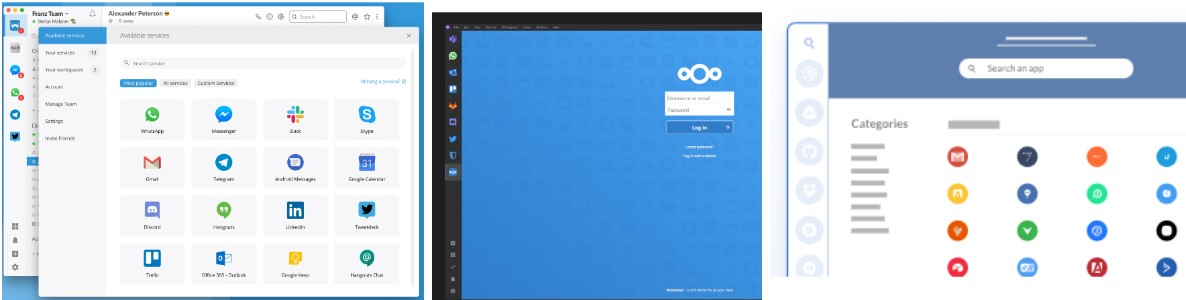
\includegraphics[width=1\textwidth]{./figuras/hub_comunicaciones.jpg}
\caption{Clientes centralizadores de comunicaciones.}
\label{F:hub_comunicaciones}
\end{center}
\end{figure}

Debido a que los clientes son un elemento variable e independiente, muchas veces se necesita tener cuentas en diversos servicios, whatsapp, telegram, teams, zoom, con el fin de tener una comunicación directa y fluida con los clientes a parte del típico formato email o llamada directa. Existen clientes hubs o centralizadores de comunicación, son aplicaciones de terceros que permiten autenticar y añadir multitud de servicios en una única interfaz funcional y simple. Permiten por ejemplo aglutinar en una app, whatsapp, telegram, slack, drive, discord. El ejemplo más conocido es Franz\cite{c_franz} software propietario con su clon opensource Ferdi\cite{c_ferdi}, o Station\cite{c_station} otro software similar. Este tipo de software es es el objetivo de nuestras necesidades por lo que es un elemento indispensable del software local, por lo que seleccionaremos comunicaciones externalizadas con elementos centralizadores como clientes.

\subsection{Servicio de interconectividad}

Después del servicio de comunicación, poderse conectarse adecuadamente entre empleados, herramientas sin ser un blanco publico de ciber-ataques, es usar una intranet, es decir, usar una VPN(virtual private network).

 Aparte de las mejoras de seguridad, geo-localización IP, filtrado y monitorización de tráfico, poder interactuar con elementos de intranet (servicios) o otros clientes conectados en formato de LAN, permite el uso de múltiples herramientas no aptas vía internet y ofrece unas mejoras sustanciales para los empleados y minimiza los problemas de configuración o acceso. 

\begin{figure}[!htb]
\begin{center}

\includegraphics[width=1\textwidth]{./figuras/intranet.jpg}
\caption{Intranet ventajas.\cite{c_intranet}}
\label{F:intranet}
\end{center}
\end{figure}
 
 El uso de acceso remoto a pc, impresoras, escáneres, ip cams, samba servers, permite en muchas ocasiones flexibilizar el trabajo físico de oficina convirtiéndolo en un remoto parcial, que puede reducir significativamente el número de horas y días físicamente en la oficina, especialmente cuando la pyme tiene una sede física de cara al público.

Por otra parte en algunos casos puede facilitar la interconexión internacional de diferentes sedes o reducir el coste de servicios internacionalizados a servicios locales por ser conducidos vía la sede internacional más local.  Un caso conocido es el uso de centralitas Asterisk\cite{c_asterisk} para el enrutado telefónico a llamadas locales/nacionales entre países,  otras veces servicios de pago pueden ser accesibles desde la intranet como por ejemplo las publicaciones científicas dentro de las red UPC.


\subsection{Servicio de almacenamiento}
Existen múltiples categorías de servicios de almacenamiento. Podemos tener discos o carpetas en red, como un servidor NFS (Network File System) o servidor samba\cite{c_samba} que nos permite acceder, editar o crear ficheros. Normalmente aunque son sencillos, dependen de una instalación previa y no están enfocados a la compartición o acceso remoto, sino al acceso a través de LAN o intranet.

Un servicio de almacenamiento-sincronizado por cliente y con página web como dropbox\cite{c_dropbox}, drive\cite{c_drive}, mega\cite{c_mega}, etc… que no solo sincroniza múltiples clientes sino que permite compartir ya sea vía cuenta o link carpetas; tener un traceado, historial, restaurar ficheros etc...

Existen multitud de ellos pero la gran mayoría de ellos tiene espacios reducidos o número máximo de clientes que limitan su funcionalidad en pequeñas empresas. Las suscripciones de pago escalan rápidamente o no están ajustadas a las demandas de una pequeña empresa o negocio por lo que no son viables económicamente 10-20 € mes con restricciones de usuarios y espacios de disco sobredimensionados.

Por último existe ecosistema que no solo almacena documentos sino que permiten interactuar con ellos, ya sea modo red social empresarial, otros servicios que acceden a los documentos (office online, drive documents).

Se entiende que un servicio equivalente a dropbox o con ecosistema es lo más apropiado para una pyme, aunque debido a la naturaleza de los recursos del VPS (poco espacio de disco), se debe usar un servidor dedicado a ello, o utilizar un proxy-redireccionador de las peticiones a servidores no limitados en espacio como puede ser una raspberry pi en la oficina o una nube autocrática. En cualquier caso, la combinación de cuentas públicas gratuitas con el servicio interno no es excluyente.

\begin{figure}[!htb]
\begin{center}
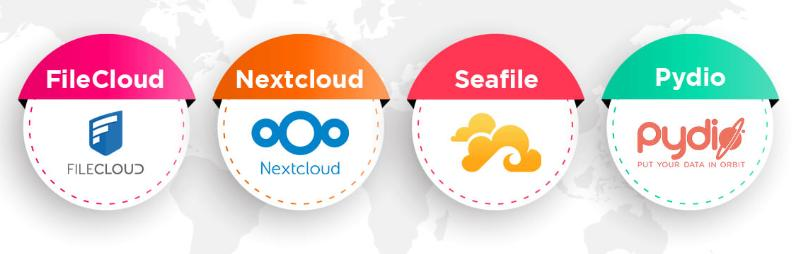
\includegraphics[width=1\textwidth]{./figuras/cloud_storage.jpg}
\caption{Opensource alternativas a almacenamiento en la nube.}
\label{F:cloud_storage}
\end{center}
\end{figure}

Se ha evaluado seafile\cite{c_seafile}, owncloud\cite{c_owncloud} y nextcloud\cite{c_nextcloud}, obteniendo un mejor resultado y satisfacción en nextcloud con una amplia integración de terceras aplicaciones y una amplia aceptación para el uso de pymes por su semejanza a plataformas gratuitas conocidas. Así mismo permite el uso de Collabora\cite{c_colabora} como onlyoffice\cite{c_onlyoffice} y su propia tool; todos herramientas de documentos en linea similar a open365 o drive documents.

Aunque requiere de un uso dedicado de recursos, es factible y económicamente viable el uso de un VPS o servidor autocrático dedicado, ya que ofrece un servicio mucho más completo, no limitado, sobre plataformas de un coste asociado reducido 4-8 € / mes, cuya finalidad no es una carga de trabajo alta, sino un servicio a un grupo reducido de usuarios.

\subsection{Servicio de documentación}
Aunque en muchos casos este servicio puede estar “camuflado” bajo servicio de almacenamiento de fichero o con terceras aplicaciones office-online, entendemos que un verdadero servicio de documentación no solo debe permitir la creación, edición y lectura de documentos sino la búsqueda, versionado e historial de los mismos.

Verdaderamente un servicio fork de wikipedia no son especialmente “densos” ni en configuración ni en recursos, por lo que son una buena práctica a utilizar. Se han evaluado 3 casos, similar a wikipedia\cite{c_media_wiki} servicio más complejo Bookstackap\cite{c_bookstack} similar a confluences o wiki de desarrollo y servicio más ligero y funcional especializados en documentación de código PineDocs\cite{c_pinedocs} que no permiten busquedas. El resultado es que cualquiera de los 3 son aptos para su uso, y debe ser una cuestión de dinámica de equipo la decisión del uso de uno de ellos o equivalente en función de si queremos una wiki interactiva publica, solo una documentación o una wiki interna.

\subsection{Servicio de Repositorios y CI}
Cuando nos referimos a entornos CI y repositorios, prácticamente la totalidad de softwares existentes pueden ser útiles, sin embargo por similitud a las plataformas privativas con cuentas gratuitas y a su interconectividad con terceras aplicaciones y plugins se han comparado una dockerización de gitlab\cite{c_gitlab}, bitbucket\cite{c_bitbucket}, gogs\cite{c_gogs} y gitea\cite{c_gitea}. El resultado ha sido que tanto gitlab como gitea son las opciones interdisciplinares y de mayor uso colectivo que son open sources y no tiene limitaciones.

\begin{figure}[!htb]
\begin{center}

\includegraphics[width=0.8\textwidth]{./figuras/ci.jpg}
\caption{Gitea junto a drone opción mas común y actual.}
\label{F:ci}
\end{center}
\end{figure}
Una buena comparativa encontramos en la propia documentación de gitea \cite{c_gitea_comparation}

Respecto a CI/CD existe un gran ganador durante los últimos 15 años que es Jenkins\cite{c_jenkins}, proyecto open source que tiene integración y documentación para ‘casi todo’ por lo que es el CI de referencia. Con el objetivo de probar otras plataforma se ha usado drone\cite{c_drone}, al ser también de uso extensivo, más moderno, pero enfocado a un CI de tamaño más reducido y configurado en los propios proyectos, es decir, que el propio desarrollador interacciona directamente con el CI sin necesidad de tener un administrador dedicado.

\subsection{Servicio de web externa}
La web externa puede ser de dos tipo estática o dinámica, aunque una web estática puede ser de utilidad para únicamente publicitar la empresa, normalmente aunque no tengan un funcionalidad concreta se tiene a usar framework dinámicos que no solo permiten ese dinamismo sino implementan estandarizaciones de temas, plugins y facilitan el mantenimiento y actualización.

 En el mundo el 43\%\cite{c_porcentaje_wordpress} de todas las web usan wordpress\cite{c_wordpress}, que es el ganador indiscutible por lo que la recomendación es clara. Sin embargo en aquellos casos de web enfocada a ventas se ha de destacar que prestashop\cite{c_prestashop} o forks opensource como thirty bees\cite{c_bees} son las maneras más automatizadas, sencillas y económicas de montar una tienda web.

Por último existe una amalgama de frameworks que generan webs estáticas via CI/CD, su principal ventaja es la ligereza, bajos recursos. Su manera de funcionar es similar a un framework dinámico, con la diferencia de que tras la realización de cambios, se compila y genera una nueva versión de la web que el ci/cd actualiza en tiempo real, un ejemplo es Hugo\cite{c_hugo}.

\subsection{Servicio de MetaDatos y contraseñas}
Existe la necesidad de dentro de un conjunto de personas que trabajan en equipo o personalmente a la hora de gestionar múltiples contraseñas, claves link y otro tipo de meta data, utilizar un gestor.
\begin{figure}[!htb]
\begin{center}
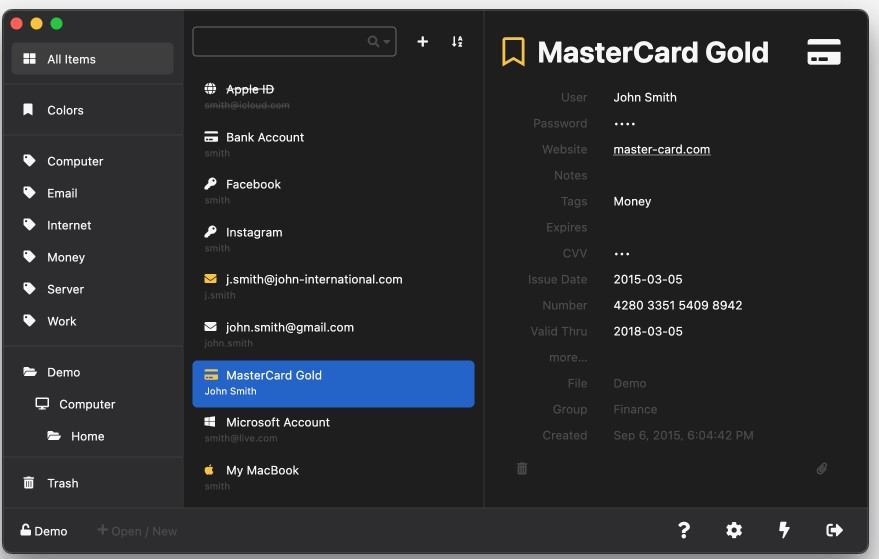
\includegraphics[width=0.8\textwidth]{./figuras/keeweb.jpg}
\caption{Gestor de metadatos y contraseñas.}
\label{F:keeweb}
\end{center}
\end{figure}
Existen gestores de nota en linea así como gestores de contraseña. Este documento aboga por la conjunción de 'profiles' en el navegador asociada a un cuenta (drive,nextcloud...) que almacena un fichero de meta-data (principalmente contraseñas), y son abiertos por KeeWeb\cite{c_keeweb} un cliente web, con aplicación de escritorio e integrado en la gran mayoría de navegadores, para acceder a documentos en la nube asociada al profile, y permitir un gestor de contraseñas, meta-data o servicios apropiadamente cifrados por una 'master-passsword'.

\subsection{Servicio de Autenticación Centralizada}
La autenticación centralizada es un mecanismo no solo de agilidad y facilidad para el cliente sino de gestión interna de usuarios y cambios centralizados de contraseña. 
\begin{figure}[!htb]
\begin{center}
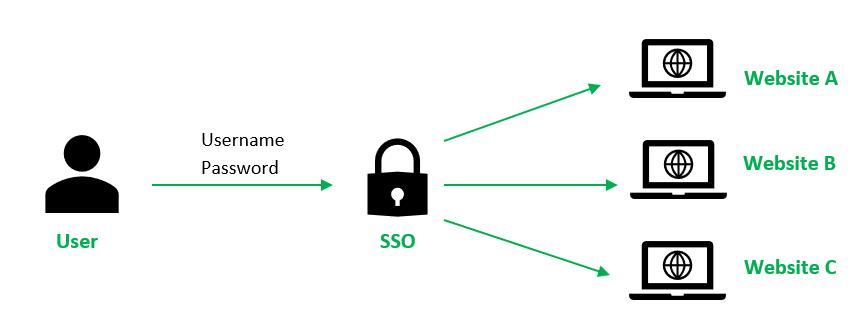
\includegraphics[width=1\textwidth]{./figuras/sso.jpg}
\caption{Single Sign on, diagrama\cite{i_sso}.}
\label{F:sso}
\end{center}
\end{figure}
Un SSO o Single Sign on (único inicio de sesión) es un mecanismo centralizado de múltiples servicios a través de un elemento centralizador. Usualmente se basa en servicios con autenticación por token a través de una API centralizadora, que genera un token al logearnos que no solo nos auténtica sino que puede incluir información extra como perfil, permisos o accesos. 

Por otra parte abre la puerta a conceptos más extensos como pueden ser el uso de identidades federadas (acceso a sistemas de terceras empresas),  Open Id, es decir proveer identidad a través de una URL, OAuth de token con acceso a recursos.

No es el objetivo de este trabajo evaluar la implementación de un SSO, pero sí realizar una prueba de concepto basada en servidor LDAP\cite{c_ldap} + Keycloak\cite{c_keycloak} , que permite realizar un ágil SSO para una pyme de más de 10 usuarios.
\begin{figure}[!htb]
\begin{center}
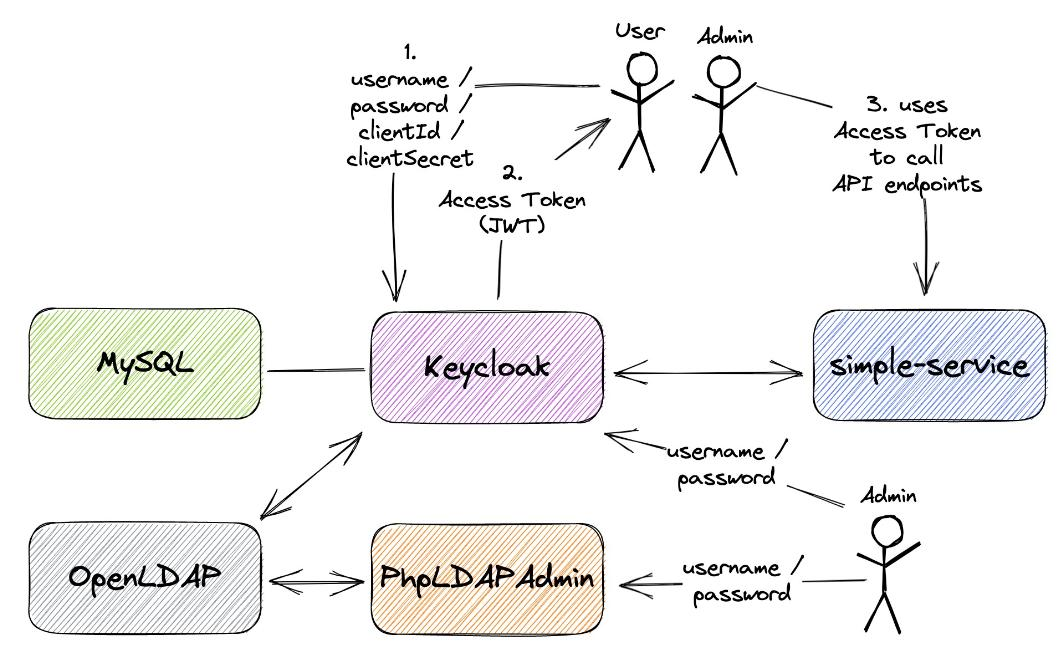
\includegraphics[width=1\textwidth]{./figuras/openldap_keycloak.jpeg}
\caption{Prueba de concepto\cite{c_openldap_keycloak} SSO Keycloak con openldap.}
\label{F:openldap_keycloak}
\end{center}
\end{figure}
Se ha probado y corroborado la prueba de concepto en anexo \ref{S:sso_example} basado en \cite{c_openldap_keycloak}, simple rápida y efectiva de Keycload + openldap que además provee de un fácil precargado de dominio ldap por fichero y comando así como un acceso UI a través de phpLdapAdmin\cite{c_php_ldap_admin}.

Actualmente muchas de las nuevas aplicaciones soportan keycloak de manera nativa a través de uno de su protocolos o vía instalación plugin, por otra parte la fuente openldap usa el protocolo ldap que es antiguo pero también ampliamente usado mecanismo de autenticación. Como concusión la practica totalidad de las aplicaciones permiten uno u otro método.

\section{Tabla de servicios públicos - externos}
Aunque se ha predefinido el uso de servicios dockerizados como principal elección, es necesario la evaluación y coste de aquellas herramientas gratuitas o externas dentro de los requisitos más inmediatos de una oficina en la nube. Se han definido una tabla de servicios y proveedores actuales para permitir evaluar su uso y coste.

\begin{center}
\label{T:externalización}
\begin{longtable}[!ht]{|p{3.25cm}|p{3.25cm}|p{3.25cm}|p{3.25cm}|}
\caption{Tabla servicios públicos para externalización.}  
\\ \hline
\textbf{Tipo de solución} & \textbf{Ventajas} & \textbf{Desventajas} & \textbf{Coste} \\ \hline
\hline
\multicolumn{1}{|c|}{\multirow{3}{*}{Correo electrónico}} &
  Google / Hotmail &
  dominio gmail/hotmail/msn &
  Gratuito \\ \cline{2-4} 
\multicolumn{1}{|p{3.25cm}|}{} &
  \multicolumn{1}{p{3.25cm}|}{gmail con dominio} &
  \multicolumn{1}{p{3.25cm}|}{no hay gratuita} &
  \multicolumn{1}{p{3.25cm}|}{5 € cuenta/año} \\ \cline{2-4} 
\multicolumn{1}{|p{3.25cm}|}{} &
  \multicolumn{1}{p{3.25cm}|}{externalizado} &
  \multicolumn{1}{p{3.25cm}|}{no hay gratuita} &
  \multicolumn{1}{p{3.25cm}|}{1-10 € / año} \\ \hline
  
\multicolumn{1}{|p{3.25cm}|}{\multirow{7}{4em}{Comunicación(real time)}} &
  \multicolumn{1}{p{3.25cm}|}{Microsoft teams} &
  \multicolumn{1}{p{3.25cm}|}{Limitaciones históricas, plugins. No administración} &
  \multicolumn{1}{p{3.25cm}|}{$\sim$5 € / mes por usuario} \\ \cline{2-4} 
\multicolumn{1}{|p{3.25cm}|}{} &
  \multicolumn{1}{p{3.25cm}|}{Zoom} &
  \multicolumn{1}{p{3.25cm}|}{Max videoconferencia 40 min. 100 Asistentes limitación mensajes.} &
  \multicolumn{1}{p{3.25cm}|}{19€ / mes usuario} \\ \cline{2-4} 
\multicolumn{1}{|p{3.25cm}|}{} &
  \multicolumn{1}{p{3.25cm}|}{Discord} &
  \multicolumn{1}{p{3.25cm}|}{Limitaciones de ficheros, histórico, enfocado a streaming} &
  \multicolumn{1}{p{3.25cm}|}{9€ / mes usuario} \\ \cline{2-4} 
\multicolumn{1}{|p{3.25cm}|}{} &
  \multicolumn{1}{p{3.25cm}|}{Slack} &
  \multicolumn{1}{p{3.25cm}|}{Historial (90 días). 10 integraciones, no Admin en canales} &
  \multicolumn{1}{p{3.25cm}|}{6.75€ / mes usuario} \\ \cline{2-4} 
\multicolumn{1}{|p{3.25cm}|}{} &
  \multicolumn{1}{p{3.25cm}|}{WhatsApp (mobile)} &
  \multicolumn{1}{p{3.25cm}|}{Requiere número móvil, usa Drive o similares como almacenamiento (15 gb)} & 
  \multicolumn{1}{p{3.25cm}|}{Gratuito} \\ \cline{2-4} 
\multicolumn{1}{|p{3.25cm}|}{} &
  \multicolumn{1}{p{3.25cm}|}{Telegram (mobile)} &
  \multicolumn{1}{p{3.25cm}|}{Requiere número móvil, no tiene gran mercado en España (como acceso a clientes)} &
  \multicolumn{1}{p{3.25cm}|}{Gratuito} \\ \cline{2-4} 
\multicolumn{1}{|p{3.25cm}|}{} &
  \multicolumn{1}{p{3.25cm}|}{Integradores de mensajería} &
  \multicolumn{1}{p{3.25cm}|}{Franz\cite{c_franz}, Rambox, Unipile software que integran desde escritorio múltiples plataformas de mensajería} &
  \multicolumn{1}{p{3.25cm}|}{Gratuito} \\ \hline
  
\multicolumn{1}{|p{3.25cm}|}{\multirow{2}{4em}{Almacenamiento y documentos en la nube}} &
  \multicolumn{1}{p{3.25cm}|}{Google - platform} &
  \multicolumn{1}{p{3.25cm}|}{Gmail o integración de tu mail con gmail} &
  \multicolumn{1}{p{3.25cm}|}{5.75€ / mes usuario} \\ \cline{2-4} 
\multicolumn{1}{|p{3.25cm}|}{} &
  \multicolumn{1}{p{3.25cm}|}{Microsoft - platform} &
  \multicolumn{1}{p{3.25cm}|}{Outlook (hotmail) o integración con tu mail} &
  \multicolumn{1}{p{3.25cm}|}{5.63 € / mes usuario} \\ \hline
  
\multicolumn{1}{|p{3.25cm}|}{\multirow{3}{4em}{Otras nubes}} &
  \multicolumn{1}{p{3.25cm}|}{NextCloud\cite{c_nextcloud}} &
  \multicolumn{1}{p{3.25cm}|}{Tecnologia opensource.} &
  \multicolumn{1}{p{3.25cm}|}{3€ / mes usuario} \\ \cline{2-4} 
\multicolumn{1}{|p{3.25cm}|}{} &
  \multicolumn{1}{p{3.25cm}|}{Dropbox\cite{c_dropbox}} &
  \multicolumn{1}{p{3.25cm}|}{Espacio limitados.} &
  \multicolumn{1}{p{3.25cm}|}{100€ / año} \\ \cline{2-4} 
\multicolumn{1}{|p{3.25cm}|}{} &
  \multicolumn{1}{p{3.25cm}|}{Owncloud\cite{c_owncloud}} &
  \multicolumn{1}{p{3.25cm}|}{Tecnología open source community y versión enterprise licenciada} &
  \multicolumn{1}{p{3.25cm}|}{Solo grandes empresas} \\ \hline
  
\multicolumn{1}{|p{3.25cm}|}{\multirow{2}{4em}{VPN o intranets}} &
  \multicolumn{1}{p{3.25cm}|}{Múltiples servicios locales no hay proveedores globales estandarizados} &
  \multicolumn{1}{p{3.25cm}|}{Se centran en intranets y redes sociales internas. No facilitan la integración en redes sino el uso online de una intranet a través de sus herramientas.} &
  \multicolumn{1}{p{3.25cm}|}{5-10 € / mes user} \\ \cline{2-4} 
\multicolumn{1}{|p{3.25cm}|}{} &
  \multicolumn{1}{p{3.25cm}|}{Solo Redes} &
  \multicolumn{1}{p{3.25cm}|}{No focalizados en empresas} &
  \multicolumn{1}{p{3.25cm}|}{3-6 € / mes} \\ \hline
  
\multicolumn{1}{|p{3.25cm}|}{\multirow{3}{4em}{Repositories y entornos CI/CD. Comparativa \cite{c_repository_comparative}}} &
  \multicolumn{1}{p{3.25cm}|}{Github\cite{c_github}} &
  \multicolumn{1}{p{3.25cm}|}{Limitación de proyectos privados y acciones ci} &
  \multicolumn{1}{p{3.25cm}|}{5€ / mes (equipo 2GB)} \\ \cline{2-4} 
\multicolumn{1}{|p{3.25cm}|}{} &
  \multicolumn{1}{p{3.25cm}|}{Gitlab\cite{c_gitlab}} &
  \multicolumn{1}{p{3.25cm}|}{Limitación de proyectos privados y acciones ci} &
  \multicolumn{1}{p{3.25cm}|}{5€ / mes full supported con 2000 ci/cd} \\ \cline{2-4} 
\multicolumn{1}{|p{3.25cm}|}{} &
  \multicolumn{1}{p{3.25cm}|}{Bitbucket\cite{c_bitbucket}} &
  \multicolumn{1}{p{3.25cm}|}{Limitación de proyectos privados y acciones ci} &
  \multicolumn{1}{p{3.25cm}|}{4€ / mes hasta 5 usuarios} \\ \hline
  
\multicolumn{1}{|p{3.25cm}|}{\multirow{3}{4em}{Web Service}} &
  \multicolumn{1}{p{3.25cm}|}{Prestashop\cite{c_prestashop}} &
  \multicolumn{1}{p{3.25cm}|}{hospedados o autogestionados} &
  \multicolumn{1}{p{3.25cm}|}{10-20 € / mes} \\ \cline{2-4} 
\multicolumn{1}{|p{3.25cm}|}{} &
  \multicolumn{1}{p{3.25cm}|}{Other custom} &
  \multicolumn{1}{p{3.25cm}|}{solo paginas webs creadas por cms} &
  \multicolumn{1}{p{3.25cm}|}{10-15 € / mes} \\ \cline{2-4} 
\multicolumn{1}{|p{3.25cm}|}{} &
  \multicolumn{1}{p{3.25cm}|}{Wordpress\cite{c_wordpress}} &
  \multicolumn{1}{p{3.25cm}|}{plugins y gestion limitada} &
  \multicolumn{1}{p{3.25cm}|}{4€ / mes} \\ \hline        
\end{longtable}
\end{center}

\textbf{Todos} los proveedores de herramientas \textbf{fidelizan} tanto a sus ecosistemas como evitan la interoperabilidad con otros, así mismo las mejores plataformas (microsoft y google) proveen de un servicio gratuito algo inferior al requerido por una pyme y a su vez no es económicamente viable usar planes business para grupos de trabajo inferiores a las 50 personas.

 La realidad es que si el ecosistema completo puede ser “barato”, una pyme no usa el 100\% de lo ofertado y el precio del pack es desproporcionado a las necesidades. Por lo tanto la implementación de soluciones opensource es la única solución que cumple nuestros requisitos de coste reducido, especialmente aquellas referidas con almacenamiento de espacio, code o intranets (vpn y definición de redes) a la vez que no excluye el uso gratuito de plataformas propietarias, como la comunicación.

\section{Servicios Dockerizados Shelf Host}
Para cada una de las necesidades virtuales existe una amalgama de servicios que suple dicha necesidad, especialmente en entornos open source. En este apartado se proponen diferentes servicios dockerizables como soluciones factibles a las necesidades más prioritarias o habituales.

En muchos de los casos existen múltiples alternativas, por lo que aquí se representan únicamente los más soportados y utilizados. En la siguiente tabla se muestran las soluciones factibles, en las cuales únicamente se han realizado pruebas de concepto en las señalados con un ‘*’. Se ha realizado la prueba de concepto aisladamente (no integrados), que permite evaluar el software y su adecuación a nuestro MVP. Verificando su funcionamientos, complejidad al instalarlo y configurarlo y recursos y agilidad de uso en el VPS.


\begin{center}
\begin{longtable}[!ht]{|p{3cm}|p{4cm}|p{6cm}|}
\caption{Tabla servicios dockerizados.}  
\label{T:servicios_dockerizados}
\\ \hline
\textbf{Tipo de Servicio} & \textbf{Herramienta} & \textbf{Detalles} \\ \hline

\multirow{6}{4em}{ Chat / Vídeo conferencia} & Rocket chat\cite{c_rocket_chat} * & Alternativa completa a slack \\ \cline{2-3} 
 & Tinode \cite{c_tinode} & Alternativa opensource \\ \cline{2-3} 
 & Zulip \cite{c_zulip} & Open source similar slack \\ \cline{2-3} 
 & Element \cite{c_element} & Open source alternativa a discord \\ \cline{2-3} 
 & Wire \cite{c_wire} & Mix de whatsapp, Telegram y signal, open source extremadamente seguro. \\ \cline{2-3} 
 & Mattermost \cite{c_mattermost} & Alternativa a slack y teams open source con integraciones de otros softwares \\ \hline

\multirow{2}{4em}{Correo electrónico} & Docker mail server\cite{c_docker_mail} & Complex but completed \\ \cline{2-3} 
 & Mailu\cite{c_mailu}* & Fácil y completo server \\ \hline
 
\multirow{2}{4em}{Autenticación Centralizada} & LDAP\cite{c_ldap}* &  Implementación de openldap, automatizadas por variables \\ \cline{2-3} 
 & Keycloak\cite{c_keycloak}* &  Federativo y contable a un ldap. \\ \hline
 
\multirow{4}{4em}{Almacenamiento y documentos en la nube} & Samba\cite{c_samba}* & Servidor de ficheros (carpetas en red) \\ \cline{2-3} 
 & Seafile\cite{c_seafile}* & Sincronización y cifrado de ficheros, simple y seguro. \\ \cline{2-3} 
 & owncloud\cite{c_owncloud}* & Clon de dropbox con add-ons, apps e integración en otros softwares \\ \cline{2-3} 
 & nextcloud\cite{c_nextcloud}* & Clon open source owncloud con mejoras y más apps. Pseudo red social y confederado. \\ \hline
 
\multirow{3}{4em}{Servicio de Documentación} & Bookstackapp\cite{c_bookstack}* &  Similar a confluence, más pesada. \\ \cline{2-3} 
 & Mediawiki\cite{c_media_wiki}* &  Equivalente a wikipedia\\ \cline{2-3} 
 & PineDocs\cite{c_pinedocs}* &  Simple ligera, perfecta para documentaciones pero no es una wiki no hay búsqueda.\\ \hline
 
\multirow{4}{4em}{VPN o intranets} & openvpn\cite{c_openvpn}* & Estándar open source actual. Complejo en cierta medida \\ \cline{2-3} 
 & wireguard\cite{c_wireguard}* & Novedoso, más fácil de usar, mejor performance \\ \cline{2-3} 
 & ipsec\cite{c_ipsec}* & estático y tiene problema con firewalls. \\ \cline{2-3} 
 & pritunl\cite{c_pritunl}* & Servidor y cliente vpn que combina múltiples protocolos incluyendo openvpn y wireguard. \\ \hline

\multirow{3}{4em}{Repositories} & gogs\cite{c_gogs}* & Servicio Git auto hospedado simple, estable y extensible, open source. \\ \cline{2-3} 
 & gitea\cite{c_gitea}* & Basado en Gogs, incluye mejoras e integraciones con terceras aplicaciones que lo equivalen a github o gitlab. \\ \cline{2-3} 
 & gitlab\cite{c_gitlab}*/ bitbucket\cite{c_bitbucket}* & tienen versiones self hosted limitadas o licenciadas. \\ \hline

\multirow{2}{4em}{CI/CD} & jenkins\cite{c_jenkins}* &  Ampliamente extendido, pero no focalizado a dockerización\\ \cline{2-3} 
 & drone\cite{c_drone}* &  especialmente enfocado a dockerización\\ \hline
 
\multirow{4}{4em}{Web Service} & wordpress\cite{c_wordpress}* & Servicio mas extendido de web (psudo dinámica)\\ \cline{2-3} 
 & prestashop\cite{c_prestashop}* / bee\cite{c_bees}* & Servicio de gran calidad para tiendas online\\ \cline{2-3} 
 & framework MVC a medida* &  Permite la creación de web dinámicas customizadas.\\ \cline{2-3} 
 & estática o framework compilado\cite{c_hugo} &  Fuente eficiente de web estáticas.\\ \hline
Ticketing & taiga\cite{c_taiga}* &  Web service para Scrum-agile.\\ \hline
 & mattermost\cite{c_mattermost}* & Gestión de comunicación y ticketing en uno. consume bastante recursos.\\ \hline
 & planka\cite{c_planka}* &   Simple Web service para Scrum-agile.\\ \hline

 \multirow{2}{4em}{DNS proxy} & mageddo\cite{c_mageddo}* &  Simple dns relay and proxy, configurable por json y interfaz gráfica.\\ \cline{2-3} 
 & simple go dns proxy\cite{c_dns_proxy_carlsverre}* &  Ejemplo de pruab de servidor dns proxy escrito en go con relay basado en docker dns.\\ \hline

\end{longtable}
\end{center}


También existe una amalgama de servicios no incluidos en el MVP conceptual pero de mayor necesidad como herramientas auxiliares para gestionar nuestra nube véase \ref{T:servicios_dockerizados_extras}

\begin{table}[!ht]
\caption{Tabla servicios dockerizados Extras.}  
\label{T:servicios_dockerizados_extras}
\resizebox{\textwidth}{!}{%
\begin{tabular}{|p{4cm}|p{4cm}|p{5cm}|}
\hline
\textbf{Tipo de Servicio} & \textbf{Herramienta} & \textbf{Detalles} \\ \hline
Gestor de contraseñas & KeeWeb\cite{c_keeweb}*/ Passbolt\cite{c_passbolt} & Un uso muy practico de gestión de contraseñas. \\ \hline
Docker UI & Portainer\cite{c_portainer}* & Un web service de despliegue de contenedores mediante UI.\\ \hline
\multirow{2}{4em}{VPN UI} & wireguard ui\cite{c_wireguar_ui}* &  Practico y eficiente UI para gestionar wireguard.\\ \cline{2-3} 
 & wg-easy\cite{c_wg_easy}* &  Sencillo UI para gestionar wireguard.\\ \hline
Monitorización y bloqueo & adguard\cite{c_adguard} home &  Servicio de bloqueo de anuncios y spam que protege tu privacidad.\\ \hline
\multirow{2}{4em}{Hub de Chat o comunicaciones} & Ferdi\cite{c_ferdi}* / Franz\cite{c_franz} * & Permite la aglutinación de los servicios más populares. \\ \cline{2-3} 
 & Station\cite{c_station} & Permite la aglutinación de los servicios más populares. \\ \hline
\end{tabular}%
}
\end{table}

Por último cabe destacar que cualquier elemento de una red empresarial tales como firewall, dhcp server, etc… todos son susceptibles de ser dockerizados e integrados en intranet, especialmente se ha hecho un uso intensibo de pruebas con ngix\cite{c_ngix} como proxy y traefik\cite{c_traefik}, así como generadores de autoridades de certificación o Let'sencrypt\cite{c_letsencrypt}.


\section{Contenedores y relaciones extendidas}\label{S:docker_compose_details}

Docker compose es una herramienta con una gran cantidad de detalles que permiten no solo agrupar y escribir en un lenguaje mas humano comando docker, sino permite setear relaciones y limitaciones de interés, tales como:
\begin{itemize}
    \item Comandos docker y sus opciones, puertos, volúmenes, variables de environment, creación e inclusión de redes etc..
    \item Dependencias de los containers especialmente a la hora de arranque, política de reinicio de containers, generación de estados o helthycheck points.
    \item Definición y restricción de recursos hardware.
    \item Imágenes, construcción de imágenes, argumentos (docker build).
    \item Labels o propiedades auto descriptivas o usadas como variables finales.
    \item Kernel parameters, para ejecutar en el container.
\end{itemize}

Por otra parte existe varias versiones de docker-compose format, existe V2\cite{c_docker_compose_v2} antigua y centrada en únicamente un host, y V3\cite{c_docker_compose_v3} una versión mas reciente con sintaxis compatible con docker-swarm que permite escalas de un único host a un cluster swarm con el mismo documento y sintaxis.

Entre otras estrategias, se puedes sobre escribir archivos o parte de los ficheros o incluir sub-ficheros para generar un docker-compose completo.

\subsection{Docker multi-capa}\label{S:docker_complex}
¿Se pueden tener un container docker con servicio docker? ¿qué es este concepto?
Por definición docker ejecuta los contenedores directamente en el sistema hospedante, pero aislando los mismos para que desde dentro sea completamente indiferente. Sin embargo si intentamos instalar docker dentro de un container docker, dicho aislamiento inhabilita la ejecución de docker ya que no tiene un control total del kernel ni de los recursos reales del servidor hostpedante.

\begin{figure}[!htb]
\begin{center}
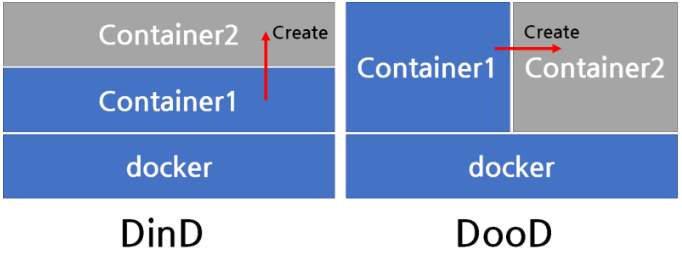
\includegraphics[width=0.7\textwidth]{./figuras/did_vs_dood.png}
\caption{Docker in docker vs Docker out of docker.}
\label{F:did_vs_dood}
\end{center}
\end{figure}

Existe tres soluciones, la denominada 'docker in docker' \cite{c_dind}, la denominada 'docker out of docker' \cite{c_dood} y la utilización de frameworks especializados como sysbox\cite{c_docker_sysbox}. En ambos casos existe una escalación o acceso a privilegios no ordinarios en un container, por lo que siempre son un posible fuente de problemas de seguridad.

Las ventajas de esta complejidad son dos, permitir una realimentación negativa de los containers y el hosts (empleada en este documento) o la creación de diferentes niveles de docker ejecutándose en paralelo en el host (de gran utilidad en CI/CD).

\subsubsection{Docker in docker (dind)}
Docker in docker o contenedores dind\cite{c_dind}, sirven para poder ejecutar docker dentro de un container. Por definición el hilo principal debe ser 'root' real para poder salir del aislamiento, lo que implica un escalado de privilegios y un gran agujero de seguridad.

\begin{figure}[!htb]
\begin{center}
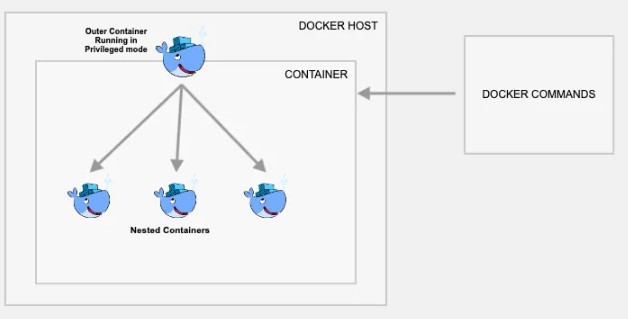
\includegraphics[width=0.7\textwidth]{./figuras/dind.jpg}
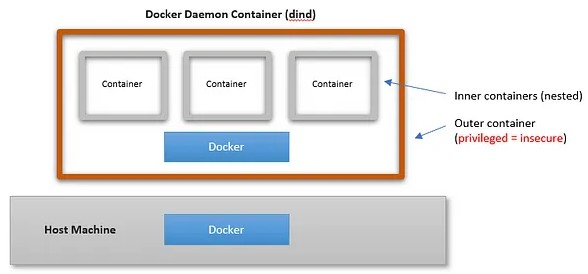
\includegraphics[width=0.7\textwidth]{./figuras/dind_command.jpg}
\caption{Docker in docker diagrama de ejecución de comandos\cite{i_dind_dood}.}
\label{F:dind}
\end{center}
\end{figure}
Con el objetivo de no comprometer el sistema hospedante vía un container con dind :
\begin{itemize}
    \item Se genera un nuevo demonio-servicio de docker, que se ejecuta exclusivamente dentro del container, por lo que no es accesible desde el sistema hospedante.
    \item Se define un nuevo usuario 'privileged' muy similar a root, que re-mapea al usuario root dentro del container. Este usuario tiene aparente root-access dentro del container, pero es un usuario con menos permisos que root del sistema hospedante, para permitir la compatibilidad se habilita un flag que permite en casos señalados escapar de su entorno namespace, para poder acceder a ciertos elementos del sistema hospedante especialmente en términos de hardware como redes, devices y particiones.
\end{itemize}
En ambos casos, los contenedores siguen ejecutándose desde el sistema hospedante, pero aquellos creados por dind, su administración se realizada por el daemon incluido en el dind container. Y siguiendo el árbol de jerarquía de procesos parando o eliminando dicho container también se acaba con todo sus subprocesos incluyendo estos contenedores adicionales no gestionados por el sistema hospedante.

La principal utilidad es la creación de contenedores temporales, especialmente en fines de CI/CD o para la ejecución de comandos vía container directamente desde dentro de un contenedor. La principal desventaja es la duplicación de espacio para la gestión de imágenes docker, al desacoplar la gestión del demonio y los posibles de ataques de seguridad directos al hardware.

\subsubsection{Docker out of Docker (dood)}
Una alternativa similar es el acceso del propio daemon docker del sistema hospedante dentro de un contenedor\cite{c_dood} y por consiguiente un acceso a la monitorización, creación o parada de contenedores, desde un propio contenedor en ejecución. De una manera similar esta realimentación negativa, debe ser controlada para evitar inestabilidades o fallos de seguridad, utilizando softwares como docker-gen\cite{c_docker_gen}, que se focalizan en las notificaciones y monitorización.
\begin{figure}[!htb]
\begin{center}
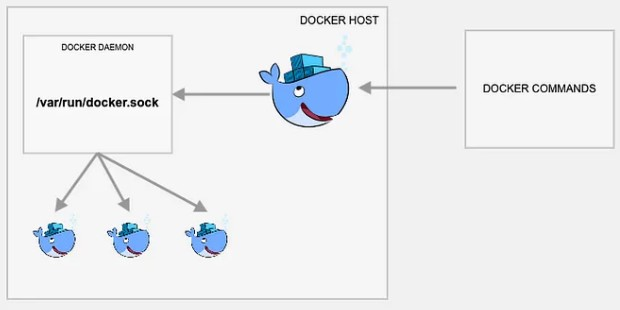
\includegraphics[width=0.7\textwidth]{./figuras/dood.jpg}
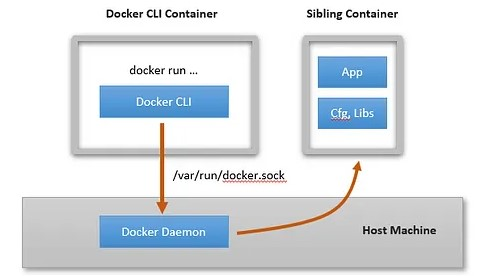
\includegraphics[width=0.7\textwidth]{./figuras/dood_command.jpg}
\caption{Docker out of docker diagrama de ejecución de comandos\cite{i_dind_dood}.}
\label{F:dood}
\end{center}
\end{figure}
Se monta en el volumen el socket del daemon de docker hospedante, sobre el mismo daemon docker en el container. Como resultado el contenedor puede acceder vía socket-daemon a información ejecutando comandos, sin incidir en riesgos de seguridad como dind.

Sus principales aplicaciones son notificaciones o monitorizaciones que automatizan muchos procesos, como son en este trabajo los proxy revers, dns-proxy automatizados y los certificados 'let's encrypt', en todos los casos un contenedor 'escanea' a sus contenedores hermanos en ejecución en paralelo y permite el acceso a datos tales como network, hostname, labels, aliases, estatus or helthycheck. En base a la información recopilada, ejecuta o genera configuraciones 'automaticas', que permiten realizar los certificados para los hostnames declarados, la redirección proxy a los mismos o el indexado dentro de nuestras rutas locales dns.

\subsubsection{Sysbox o equivalentes}
Existen frameworks de trabajo como Sysbox\cite{c_docker_sysbox} que proporcionan un entorno de ejecución equivalente a dind, pero sin la necesidad de utilizar los flag de privilegios.
\clearpage
\begin{figure}[!htb]
\begin{center}
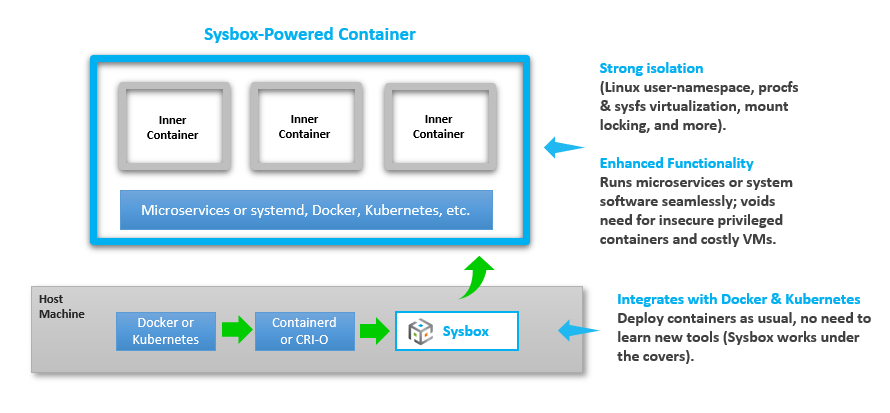
\includegraphics[width=1\textwidth]{./figuras/sysbox-diagram.png}
\caption{Sysbox \cite{c_docker_sysbox} diagrama de funcionamiento.}
\label{F:sysbox-diagram}
\end{center}
\end{figure}
Esta es la solución mas innovadora y relevante, ya que la misma compañía de docker ha comprado a sysbox el pasado año. Sin embargo muchos de los imágenes docker utilizadas en este documento requieren de un soporte comunitario para su mantenimiento, que aun no ha sido migrado a ejecuciones bajo sysbox.

\subsection{SystemD service con docker-compose}\label{S:systemD}
Una vez que tenemos un grupo de servicios definidos, automatizados dentro de un docker-compose con ciertos scripts, podemos decir que tenemos unos 'servicios dockerizados' en funcionamiento. Sin embargo para el sistema hospedante no dejan de ser unos procesos arbitrarios como comandos que podemos ejecutar dentro de una terminal. Cuando reiniciamos el servidor o se enciende después de un apagado dichos procesos han muerto y sido eliminados.

Definir dichos servicio/servicios como un servicio o modulo de systemD\cite{c_systemd} no solo aporta valor de cara a estandarizar dentro del sistema linux dichos servicios sino que permite automatizar, reinicio, modos de mantenimiento y arranque del servicio de una manera mas automática y estándar.

Se puede optar por un script genérico que ejecuta los servicios de docker desde un modulo de systemD (customizado), basado en argumento '\%i' pasado al modulo para ejecutarse sobre diferentes sub-carpetas cada una con el docker-compose del servicio (véase \ref{lst:docker_compose_systemD_module}).

\begin{lstlisting}[language=bash, caption={SystemD /etc/systemd/system/docker-compose@.service}, label={lst:docker_compose_systemD_module} ]
[Unit]
Description=%i service with docker compose
PartOf=docker.service
After=docker.service

[Service]
Type=oneshot
RemainAfterExit=true
WorkingDirectory=/yourFolderwithService/group_services/%i
ExecStartPre=/usr/local/bin/docker-compose pull --quiet --parallel
ExecStart=/usr/local/bin/docker-compose up -d
ExecStop=/usr/local/bin/docker-compose down
ExecReload=/usr/local/bin/docker-compose pull --quiet --parallel
ExecReload=/usr/local/bin/docker-compose up -d

[Install]
WantedBy=multi-user.target
\end{lstlisting}

Por otra parte también se pueden automatizar tanto la actualización de imágenes de docker (al basarse en LTS continuamente mantenidos por su comunidad), llamando a un 'Reload' del servicio. Como alternativa definir un servicio customizado de SystemD por cada servicio o agrupación de servicios apuntando a un docker-compose o un script customizado (véase \ref{lst:systemD_custom}). Ambas opciones pueden ser puestas en marcha a la vez, sin embargo hay que tener en cuenta la interacción entre las mismas.

\begin{lstlisting}[language=bash, caption={SystemD /etc/systemd/system/custom-service}, label={lst:systemD_custom} ]
[Unit]
Description=docekrrized services manage by scripting and docker-compose
PartOf=docker.service
After=docker.service

[Service]
Type=oneshot
RemainAfterExit=true
WorkingDirectory=/yourFolderwithYourScripts
ExecStart=./start.sh 
ExecStop=./stop.sh 

[Install]
WantedBy=multi-user.target
\end{lstlisting}

Por ultimo remarcar que la ejecución de ciertas tareas puede automatizarse mediante 'cron' \ref{lst:cron_docker_reload} o directamente usando systemD \ref{lst:systemD_timer_docker_reload} \ref{lst:systemD_docker_reload}

\begin{lstlisting}[language=bash, caption={Crone line /etc/crontab, actualizacion imagenes}, label={lst:cron_docker_reload} ]
0  4    * * *   root    /bin/systemctl reload docker-compose@*.service
\end{lstlisting}

\begin{lstlisting}[language=bash, caption={SystemD /etc/systemd/system/docker-compose-reload.timer}, label={lst:systemD_timer_docker_reload} ]
[Unit]
Description=Refresh images and update containers
Requires=docker-compose.service
After=docker-compose.service

[Timer]
OnCalendar=*:0/15

[Install]
WantedBy=timers.target
\end{lstlisting}

\begin{lstlisting}[language=bash, caption={SystemD /etc/systemd/system/docker-compose.reload.service }, label={lst:systemD_docker_reload} ]
[Unit]
Description=Refresh images and update containers

[Service]
Type=oneshot

ExecStart=/bin/systemctl reload docker-compose@*.service
\end{lstlisting}

Utilizando una aproximación similar podemos centralizar los mecanismos de mantenimiento o backup de los diferentes servicios dockerizados via 'cron-script' o 'systemD service-timer'.

Por ultimo si se desea poder acceder a los logs de los nuevos servicios systemD\cite{c_systemd} desde la plataforma de 'journald'\cite{c_journald} se debe indicar en la configuración de docker el driver de log apropiado:
\begin{lstlisting}[language=json, caption={Fichero de configuracion daemon.json}, label={lst:docker_log_journald} ]
{
  "log-driver": "journald"
}
\end{lstlisting}


\subsection{Backups y restauración de servicios}
Con el fin de realizar los backups se asumido una gestión por scripting o systemD, el principal objetivo es mediante un timer o cron que ejecuta un proceso de apagado de servicios dockerizados y realizar el backup a una horas poco usuales, como puede ser 2-4 de la noche.
\begin{figure}[!htb]
\begin{center}
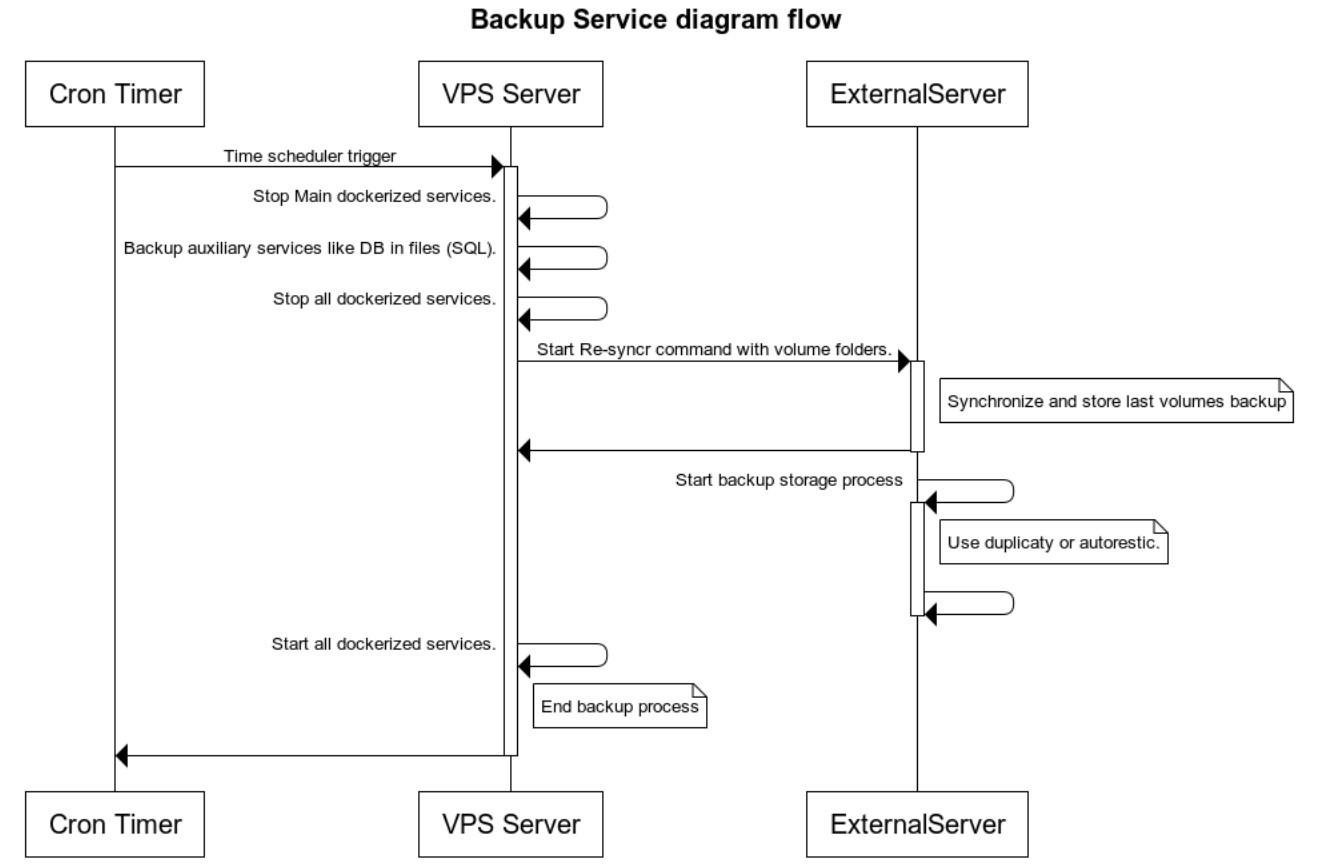
\includegraphics[width=1\textwidth]{./figuras/backup_diagram}
\caption{Backup diagrama de secuencia.}
\label{F:backup_diagram}
\end{center}
\end{figure}
Como existe una limitación de espacio y de CPU en el VPS, pero no tenemos trafico intenso en las VPS o el VPS durante el periodo nocturno la solución ha sido externalizar el proceso de backup, entendido como almacenamiento de versiones con historial a un servidor externo, que puede perfectamente pertenecer a la VPN (ser autócrata).
Por lo tanto el proceso de backup únicamente realiza una sincronización de carpetas y ficheros con el servidor externo, es decir, en muchos casos servicios que no realizan cambios de manera continuada como el VPN server, pueden ser sincronizados sin necesidad de apagado. Por otra parte es en el servidor externo donde se configura apropiadamente la gestión de backups, donde no tenemos limitaciones de CPU o espacio en disco y se utilizaran herramientas que permiten el almacenamiento de un históricos basados en tags o identificadores y en diferencias entre versiones de una manera similar a git. El objetivo se basa en como en git, permitir un almacenaje reducido, poder acceder a versiones especificas por fecha o identificador, añadir una capa de redundancia, checksum o incluso cifrado al almacenamiento de los backups.
\begin{figure}[!htb]
\begin{center}
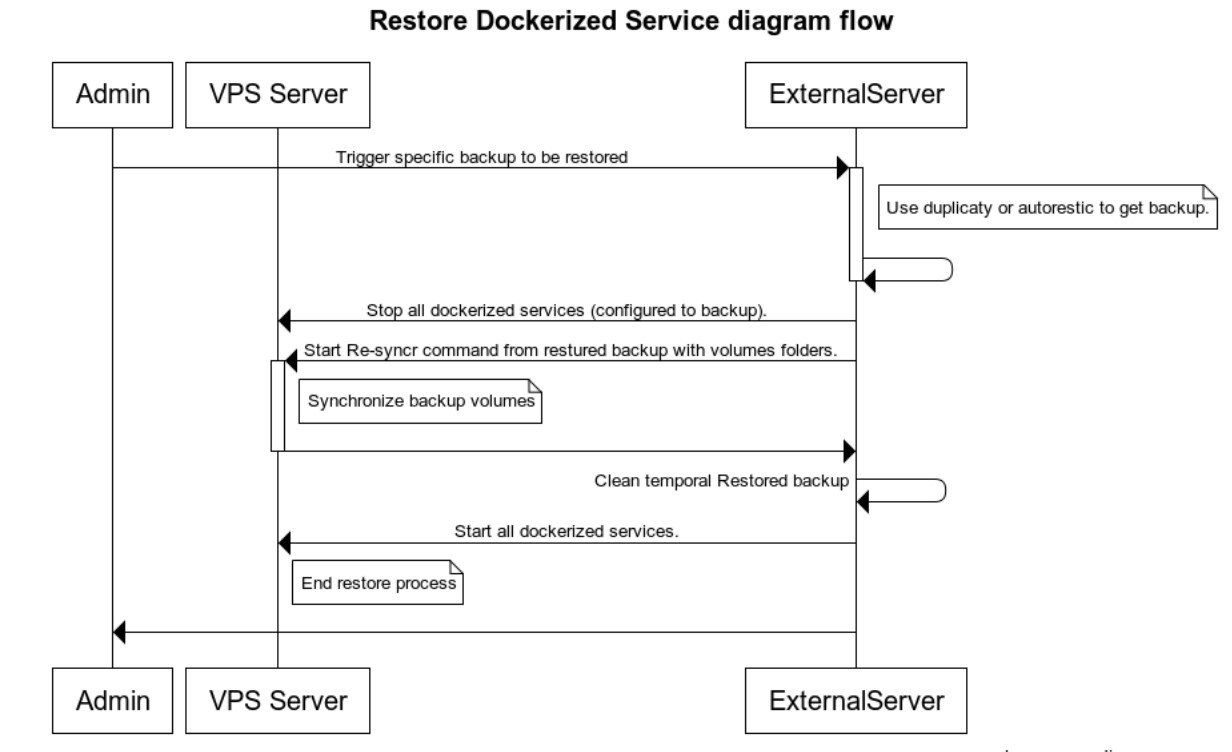
\includegraphics[width=1\textwidth]{./figuras/restore_diagram}
\caption{Restore diagrama de secuencia.}
\label{F:restore_diagram}
\end{center}
\end{figure}
Por otra parte la lógica de restauración funciona de manera inversa, puesto que una restauración no es automática, sino que es iniciada por el administrador, inicializa el servidor externo para preparar el backup especifico. Una vez generado el backup requerido se procede a la parada de los servicios docker en el VPS y una posterior sincronización inversa servidor externo - VPS para finalmente volver a arrancar los servicios véase figura \ref{{F:restore_diagram}.


\subsection{Estructura de ficheros}
La estructura de ficheros y docker-compose debe ser coherente y ágil para realizar backups, declarar servicios systemD o permitir el arranque, parada o actualización local de grupos de containers. Se han probado diferentes soluciones durante la realización de este trabajo, aunque no se ha definido 'la mejor manera de trabajar' y simplemente queda mostrada varios casos para que el administrador use la mas adecuada a sus necesidades.

Por una parte es importante definir una carpeta principal sobre la que trabajar, en esta carpeta contiene un docker-compose general con todos los servicios, carpetas de volúmenes compartidos por uno o mas servicios, o contraseñas token segurizados correctamente mediante secrets.
Debido al gran numero de servicios, redes y otras propiedades, es probable que se separen diferentes grupos de contenedores, en base a servicios principales y auxiliares de estos servicios principales (figura \ref{F:DockerServiceFolder}).
\begin{figure}[!htb]
\begin{center}
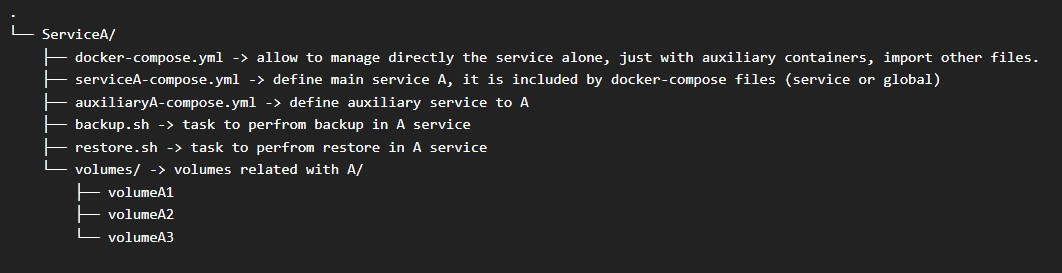
\includegraphics[width=1\textwidth]{./figuras/DockerServiceFolder}
\caption{Estructura de un Servicio A.}
\label{F:DockerServiceFolder}
\end{center}
\end{figure}

\begin{figure}[!htb]
\begin{center}
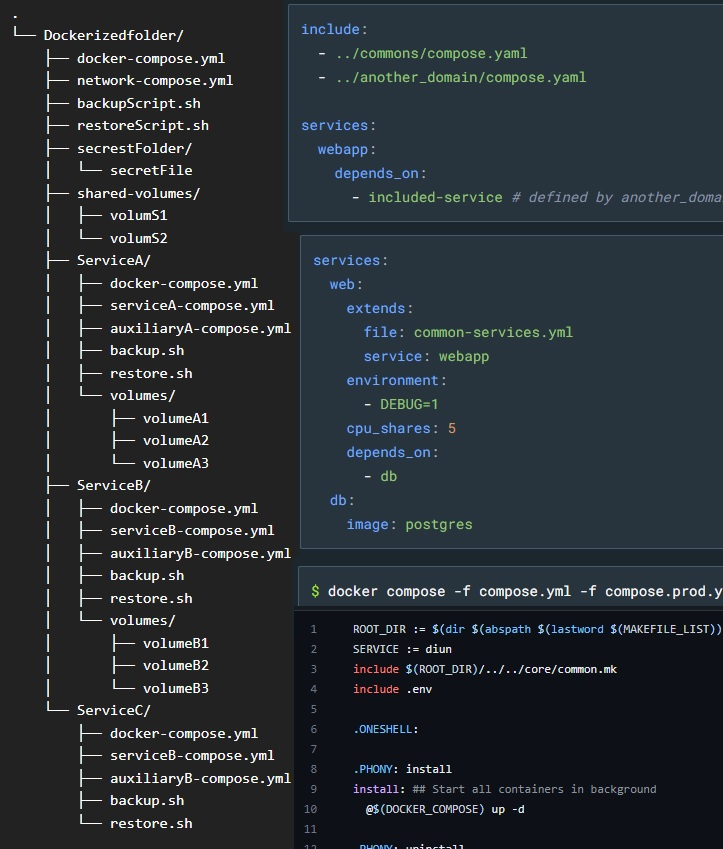
\includegraphics[width=0.8\textwidth]{./figuras/Ejemplos_estrcutura}
\caption{Estructura completa y ejemplos de include, merge o makeFile.}
\label{F:Ejemplos_estrcutura}
\end{center}
\end{figure}
Para la gestión de los servicios se puede optar por un script 'services.sh' o como se ha indicado en \ref{S:systemD} un servicio SystemD, en ambos casos la estructura de subcarpetas por servicio principal, nos permite auto-gestionar por argumento '\%i' el servicio en cuestión, o aplicar comandos al conjunto de ellos ('i = *').

Utilizar las funcionalidades de 'include'\cite{c_docker_compose_include} y 'merge'\cite{c_docker_compose_merge} puede permitirnos definir en diferentes fichero aquellos elementos globales (redes, volumen compartido), como los servicios principales y sus auxiliares, permitiendo definir las funcionalidades en un único fichero que es posteriormente incluido en un docker-compose.

El concepto es permitir gestionar autonómicamente el servicio principal, ya sea desde su docker-compose desde la sub-carpeta ServicioA, o directamente desde el conglomerado de servicios de la carpeta principal.

Por ultimo, existen los script de 'backup.sh' y 'restore.sh' realizar dichas tarea de manera reiterativa sobre los subfolder y scripts de cada servicio. O por una temática similar a bash script, archivos makeFile, con comandos de instalación, arranque, parada, backup y restauración, equivalentes muy similar.

Se tiene que comprender, que dependiendo de las necesidades y especialmente del numero de servicios, una nube mas compleja, requerirá de una segmentación mas clara, y una estructura jerárquica mas definida. Por ejemplo podemos definir nuestros servicios dockerizados tal y como muestra el ejemplo, e incluirlo en un proyecto de git, que excluya aquellos volúmenes variables (con datos), y folders sensibles como secrets. De esta manera podemos guardar nuestra 'backup de configuración' sin datos asociados a un proyecto fácilmente desplegable vía ansible.

Otro ejemplo puede ser similar a mars-server\cite{c_mars_server}, pre-configurar el caso mas complejo, y únicamente habilitar o 'instalar' aquellos servicios que realmente deseemos utilizar dentro del servidor.

En todo caso la opción mas apropiada seria la generación de un aplicativo capaz de aglutinar las diferentes pruebas de concepto de este trabajo, y generar dinámicamente vía ui, los docker-compose o ficheros a utilizar, así como una gestión mas intuitiva. Desgraciadamente debido a limitaciones de recursos y tiempo no ha sido objetivo dentro de este documento, aunque probablemente se materialice durante 2024.
